\documentclass{article}
\usepackage[utf8]{vietnam}
\usepackage{amsthm}
\usepackage{amsmath}
\usepackage{amsfonts}
\usepackage{amssymb}
\usepackage{graphicx}
\usepackage{url}
\usepackage{cases}

\title{\textbf{Phân tích thiết kế hệ thống "Đăng ký môn học"}}
\author{
  Ngô Quang Dương\\
  Hà Thế Lực\\
  Nguyễn Thanh Tuyên
}
\date{\today}

\begin{document}

\maketitle

\begin{abstract}
\end{abstract}

\section{Mở đầu}

  \subsection{Đặt vấn đề}

  \subsection{Hệ thống hiện tại}

  \subsection{Hướng giải quyết}

\section{Thu thập và phân tích yêu cầu}
  
  \subsection{Bảng thuật ngữ}
  
  \subsection{Tác nhân hệ thống}
    \begin{itemize}
      \item Sinh viên.
      \item Chuyên viên phòng đào tạo.
      \item Giảng viên.
      \item Người quản trị hệ thống.
    \end{itemize}
  
  \subsection{Yêu cầu chức năng}
    \paragraph{
      \textnormal{
        Chức năng chung:
      }
    }
    \begin{itemize}
      \item Đăng nhập/đăng xuất.
      \item Tìm kiếm.
      \item Xem thông tin môn học.
    \end{itemize}

    \paragraph{
      \textnormal{
        Chức năng dành cho sinh viên:
      }
    }
    \begin{itemize}
      \item Đăng ký môn học.
        \begin{itemize}
          \item Đăng ký môn mới.
          \item Hủy đăng ký.
        \end{itemize}
      \item Xem kết quả đăng ký.
      \item In kết quả đăng ký học.
    \end{itemize}

    \paragraph{
      \textnormal{
        Chức năng dành cho chuyên viên:
      }
    }
    \begin{itemize}
      \item Thay đổi kết quả đăng ký học của sinh viên.
      \item Xem kết quả đăng ký của sinh viên.
      \item Xem thông tin sinh viên.
    \end{itemize}

    \paragraph{
      \textnormal{
        Chức năng dành cho giảng viên:
      }
    }
    \begin{itemize}
      \item Chọn lớp môn học.
      \item Quy định số sinh viên tối đa/tối thiểu được đăng ký.
    \end{itemize}

    \paragraph{
      \textnormal{
        Chức năng dành cho người quản trị hệ thống:
      }
    }
    \begin{itemize}
      \item Đóng/mở đăng ký học.
      \item Lập thời khóa biểu.
      \item Thay đổi thời khóa biểu.
      \item Quản lý người dùng:
      \begin{itemize}
        \item Tạo người dùng mới.
        \item Thay đổi thông tin người dùng.
        \item Xóa người dùng.
      \end{itemize}
    \end{itemize}

  \subsection{Yêu cầu phi chức năng}
    \paragraph{
      \textnormal{
        Qua khảo sát của hai kiểu người dùng là sinh viên và giảng viên, về mặt phi chức năng cần đáp ứng các yêu cầu sau:
      }
    }
    \begin{itemize}
      \item Kết nối nhanh.
      \item Thời gian thực.
      \item Giao diện dễ sử dụng.
      \item Dễ tìm kiếm môn học cần đăng ký.
    \end{itemize}
  
  \subsection{Điều kiện ràng buộc}
    
    \paragraph{\textnormal{
      Đối với sinh viên:
    }}
    \begin{itemize}
      \item Không đăng ký quá 2 môn giáo dục thể chất.
      \item Không đăng ký các môn học có kết quả trên $D$.
      \item Số tín chỉ tối thiểu:
      \begin{itemize}
        \item Chương trình chuẩn: $14$.
        \item Chương trình chất lượng cao: $16$.
        \item Chương trình chuẩn quốc tế: $16$.
        \item Chương trình đào tạo tài năng: $18$.
      \end{itemize}
    \end{itemize}

    \paragraph{\textnormal{
      Đối với quản trị hệ thống:
    }}
    \begin{itemize}
      \item Không có buổi học nào trùng cả phòng học lẫn giờ học.
      \item Không tự ý thay đổi thông tin của người dùng.
    \end{itemize}

\section{Đặc tả yêu cầu}

  \subsection{Sơ đồ use case}
    \begin{figure}[!ht]
      \centering
      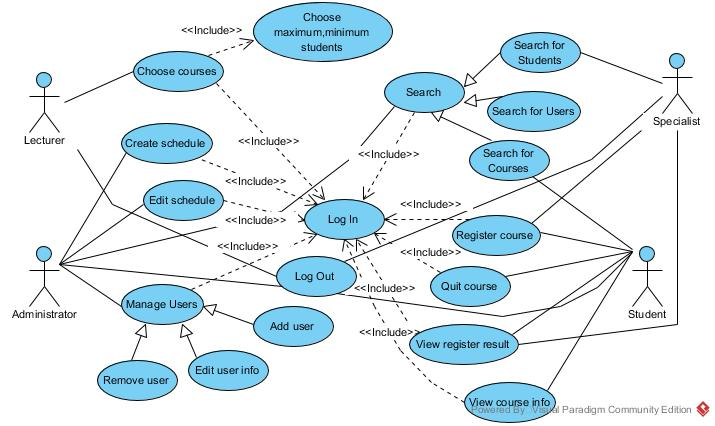
\includegraphics[scale=0.4]{../pictures/projectdiagrams/usecasediagram.jpg}
      \caption{Sơ đồ use case của hệ thống đăng ký môn học}
    \end{figure}

  \subsection{Đặc tả use case}

  \subsection{Sơ đồ hoạt động}

\section{Phân tích tĩnh}

  \subsection{Xác định lớp}

  \subsection{Quan hệ giữa các lớp/sơ đồ lớp}

  \subsection{Lớp phân tích}

  \subsection{Xác định thuộc tính}

  \subsection{Xác định phương thức}

\section{}

\end{document}
